
\subsection{Convex hull of images and efficiency}

%TODO: Describe and explain the efficiency of different cases,
%and potential solutions for problematic areas.
%Remember graphical illustrations.

As explained in the section regarding pixel-perfect
collision detection as well as elsewhere,
the more accurate a convex hull is in regards to its
corresponding binary image, the more efficient
collision detection is going to be.

The efficiency of pixel-perfect collision detection
is affected somewhat by transformations.
The basis is that the efficiency changes from transformation is only
affected by the change in area.
The reason is that the larger the area, the more pixels
will have to be checked.
For instance, if a 1-by-1 image, containing 1 pixels,
is scaled by a factor of 100 in both direction,
100 * 100 = 10.000 pixels will have to be checked
in the worst-case
(assuming that the intersection actually covers all
those pixels, and no 'hits' are found early).
That means that rotation and translation are free;
meaning that they do not have any effect
on the efficiency of pixel-perfect collision detection.
Scaling, on the other hand, can either increase
or decrease the efficiency, with enlarging scaling
decreasing the efficiency, and contriction
increasing it.
Note that these considerations only goes for
image primitives. Transformation does not
affect the efficiency of polygon v. polygon
collision detection.

Overall, if at least one of the primitives is
based on a binary image, the intersection
size and how early a 'hit' occurs on average
(assuming some reasonable random distribution of collisions)
determines the efficiency. Accuracy is the main determinant
in how early hits occur.

One possibility for certain images with low precision is
splitting them into smaller parts, where the smaller parts
are much better approximated by a convex hull.
Splitting creates more collision objects, which generally
decreases performance, which means that splitting is not
a silver bullet; but for a considerable number of cases,
a few splits can increase the precision a large amount.

In the following part, different examples of
images and convex hulls are going to be investigated, show-casing
which kind of images will be efficient,
which kind of images will not be efficient,
and what methods are available to increase
efficiency.

Figure \ref{fig:image_perfect} shows a binary image
(black indicates 'on' pixels, white indicates 'off'
pixels) with a convex hull (marked by blue).
The area covered by the convex hull is precisely the
same as the binary image, which means the accuracy
is $100\%$. Since the binary image is approximated perfectly
by the convex hull, it might make sense in this case
to simply use the convex hull as the primitive.
But it does not change much in practice,
and using the image as the primitive instead
of the convex hull may be more convenient.
The efficiency should be about the same as
if it was using the convex hull for collision detection.

Figure \ref{fig:image_nearperfect} shows a near-perfect image.
Since the convex hull is not $100\%$ accurate, it cannot be replaced
by a convex hull without loss of precision. However, it is still quite
efficient, since the difference in terms of area between the convex hull
and the image is very small.

Figure \ref{fig:image_roundedcorners} shows a rectangle with rounded corners.
In practice, the convex hull will have several points to help cover the corners,
and the larger the image, the more points it will have for the corners.
The number of corners should in practice not pose a problem,
and since the area of the image and the convex hull are very nearly the same,
the precision is good as well.

Figure \ref{fig:image_ok} shows an image that is ok in regards to precision.
There is a small, but significant difference in area between the convex hull
and the image. As long as the image itself is small, this image should perform
reasonably, but if the image is larger, it may not perform very efficiently
in corner cases.

Figure \ref{fig:image_singlesplit} shows an image that is bad in regards
to precision. In this case the precision can easily
become optimal simply by splitting the image once in the right place.
The right place is indicated by a red, dashed line in the image.
Whether it is worth splitting it depends on whether the performance
of the original image is worth the extra amount of work required
to split it.

Figure \ref{fig:image_ring} shows an image of a ring.
This image has very low precision due to the large difference in area
between the convex hull and the ring.
One way to increase the precision considerably would be to split the image repeatedly,
for instance into 8 parts that cover an equal part of the ring,
meaning that much of the large empty area in the middle would not be covered
by the convex hull to the same degree as if not splitting.
This does, however, introduce 8 new parts.

Figure \ref{fig:image_complex} shows a large and complex image.
The image has low precision, but it is difficult and requires much work
to split well. Furthermore, any high-precision split would produce many
different parts. Assuming that the difficulty and effort required to split
the image is acceptable, is it more efficienct to split such an image?
Since the image is so large, it very likely will be, since precision
is more important the larger the image is.

The final figure to consider is figure \ref{fig:image_cloud}.
The cloud has low density and uniform distribution,
and the precision is low. Even splitting will not help a lot here,
because the number of parts needed to really increase the precision
is close to the number of pixels, which is very inefficient, and likely
to be much less efficient than just a single convex hull.
This image can be considered a sort of 'worst-case' for the library,
since it is difficult to handle it efficiently.
Whether this is a problem depends on the context the library is deployed in.

\begin{figure}[p]
	\centering
	\begin{subfigure}[b]{0.3\linewidth}
	  \centering
	  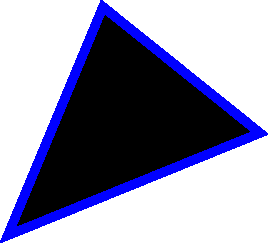
\includegraphics[scale=0.5]{convexhullimages/image_perfect.pdf}
	  \subcaption{Perfect image}
	  \label{fig:image_perfect}
	\end{subfigure}
	\centering
	\begin{subfigure}[b]{0.3\linewidth}
	  \centering
	  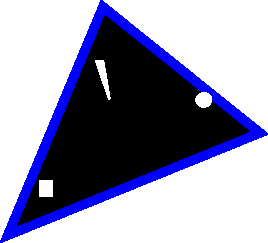
\includegraphics[scale=0.5]{convexhullimages/image_nearperfect.pdf}
	  \subcaption{Near-perfect image}
	  \label{fig:image_nearperfect}
	\end{subfigure}
	\centering
	\begin{subfigure}[b]{0.3\linewidth}
	  \centering
	  
\includegraphics[scale=0.5]{convexhullimages/image_roundedcorners.pdf}
	  \subcaption{Image of rectangle with rounded corners}
	  \label{fig:image_roundedcorners}
	\end{subfigure}
	\centering
	\begin{subfigure}[b]{0.3\linewidth}
	  \centering
	  
\includegraphics[scale=0.5]{convexhullimages/image_ok.pdf}
	  \subcaption{Ok image}
	  \label{fig:image_ok}
	\end{subfigure}
	\centering
	\begin{subfigure}[b]{0.3\linewidth}
	  \centering
	  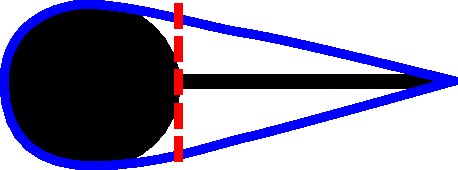
\includegraphics[scale=0.5]{convexhullimages/image_singlesplit.pdf}
	  \subcaption{Image with bad precision which can be fixed by a single split}
	  \label{fig:image_singlesplit}
	\end{subfigure}
	\centering
	\begin{subfigure}[b]{0.3\linewidth}
	  \centering
	  
\includegraphics[scale=0.5]{convexhullimages/image_ring.pdf}
	  \subcaption{Image of a ring with very low precision}
	  \label{fig:image_ring}
	\end{subfigure}
	\centering
	\begin{subfigure}[b]{1.0\linewidth}
	  \centering
	  
\includegraphics[scale=0.7]{convexhullimages/image_complex.pdf}
	  \subcaption{Large, complex image that has low precision and which is difficult to split manually}
	  \label{fig:image_complex}
	\end{subfigure}
	\centering
	\begin{subfigure}[b]{0.3\linewidth}
	  \centering
	  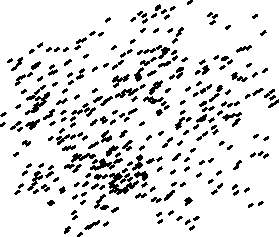
\includegraphics[scale=0.5]{convexhullimages/image_cloud.pdf}
	  \subcaption{Image of a cloud, with very low precision and uniform distribution}
	  \label{fig:image_cloud}
	\end{subfigure}
\caption{Images and convex hulls}
\label{fig:convexhullimages}
\end{figure}

Splitting images can be a difficult and laborious process.
One possible extension to the library would be an automatic splitting algorithm,
that tries to increase the precision with as few different parts as possible.
It should be possible to create such an algorithm that works reasonably well
for many different contexts, but it has not yet been provided in the library.

One possibility is taking the image, finding the longest length, and split the image
in half. Then take the convex hull of each part, and determine how precise each
part is. If the part is not precise enough, the process is repeated recursively for the part.
To avoid recursion, the process stops if the number of parts become too large, or the image
to split becomes too small.
The precision threshold, the number of part to accept (possibly dependent on the image size),
and the size of image to stop at are heuristics that has to be determined somehow
(either manually through testing or automatically through some machine learning and regression
testing).

